\documentclass[11pt]{article}
\usepackage[margin=0.9in]{geometry}
\usepackage{amsmath,amssymb,amsthm,mathtools}
\usepackage{booktabs,array,longtable}
\usepackage{tikz}
\usetikzlibrary{arrows.meta,positioning,calc}
\usepackage{microtype}
\usepackage{hyperref}
\hypersetup{colorlinks=true,linkcolor=blue!55!black,citecolor=blue!55!black,urlcolor=blue!55!black}
\newtheorem{theorem}{Theorem}[section]
\newtheorem{proposition}[theorem]{Proposition}
\newcommand{\Sset}{\mathcal C}
\title{\textbf{Discrete Settlement Tensors and Constrained Optimization in DATA 3.0 / AMLD}\\[4pt]\large Settlement Density, One-Hot Terminal States, and Resource Allocation}
\author{Brian Tenneson}
\date{August 13, 2026}
\begin{document}
\maketitle

\begin{abstract}
A multi-agent conjecture settler must decide where finite computation should go before any terminal certificate has been found. This note distinguishes actual settlement from predictive navigation quantities, introduces a discrete settlement tensor for direct, lemma, and cross-agent value, and formulates resource allocation as a constrained optimization problem. Under standard compactness and concavity assumptions, optimal allocations exist and KKT conditions characterize global optima. Strict or strong concavity gives uniqueness and stability. A simple diminishing-returns model yields an explicit water-filling scheduler. Uniform error in an estimated settlement objective produces a quantitative $2\varepsilon$ near-optimality guarantee. These results address a meta-level optimization problem; they do not imply that arbitrary mathematical targets are decidable.
\end{abstract}

\section*{AI Integrity Statement}
Brian Tenneson is the author of this manuscript and is responsible for its mathematical claims, interpretation, and release. OpenAI ChatGPT was used as an AI research and drafting consultant for mathematical formalization, literature search, exposition, figure design, and LaTeX preparation. No theorem or experimental claim is accepted solely because it was suggested by an AI system. Formal claims are intended to stand on explicit definitions, assumptions, and proofs. Experimental claims require frozen protocols, retained search data, and verifier-backed certificates. Proposed AMLD terminology and architecture remain research proposals unless independently validated.

\section{Actual settlement is mutually exclusive}
For a target $w$ over a frozen base theory $T$, let
\[
\Sset_P,\qquad \Sset_R,\qquad \Sset_I,\qquad \Sset_C
\]
be terminal certificate classes for proof, refutation, independence, and contradiction. The contradiction class means that both $w$ and $\neg w$ have been certified in the declared base/context. The terminal classes are required to be pairwise disjoint.

Define certified settlement indicators
\[
S_k(x)=\mathbf 1\{x\in\Sset_k\},\qquad k\in\{P,R,I,C\}.
\]
Then
\[
\boxed{S_P(x)+S_R(x)+S_I(x)+S_C(x)\le 1.}
\]
At a settled state exactly one coordinate is $1$; before settlement all four actual-settlement indicators are $0$. Fractional quantities such as $F_P,F_R,F_I,F_C$ are predictions or navigation measurements, not terminal states.

\section{What settlement density means}
The phrase \emph{settlement density} is proposed terminology. It means the weighted amount of certificate-relevant verified information found per unit search volume or computational cost. A region containing many easy but irrelevant lemmas can have lower settlement density than a sparse region containing one lemma that sharply reduces the remaining proof, refutation, or independence horizon.

A schematic local density for certifier $k$ is
\[
\rho_k(x)=\frac{\sum_{y\in N(x)}w_k(y)\,\mathbf 1\{y\text{ is verified and useful to }k\}}{\operatorname{Vol}(N(x))}.
\]
The weight $w_k(y)$ measures settlement relevance rather than mere theoremhood.

\begin{figure}[ht]
\centering
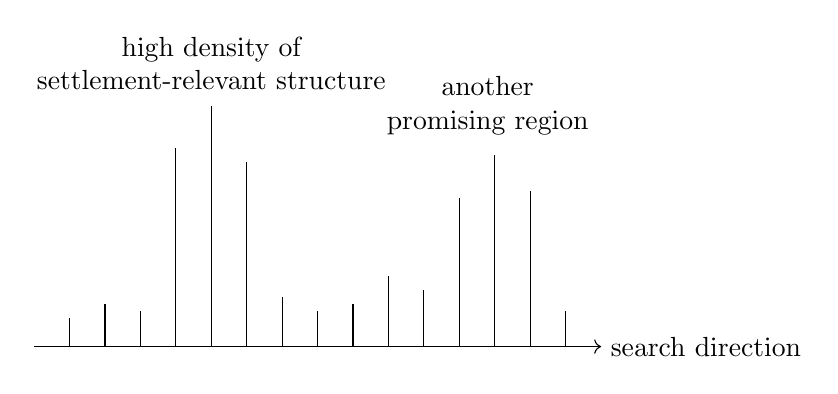
\begin{tikzpicture}[x=0.9cm,y=0.9cm]
\draw[->] (0,0)--(8,0) node[right]{search direction};
\foreach \x/\h in {0.5/0.4,1/0.6,1.5/0.5,2/2.8,2.5/3.4,3/2.6,3.5/0.7,4/0.5,4.5/0.6,5/1.0,5.5/0.8,6/2.1,6.5/2.7,7/2.2,7.5/0.5}{\draw (\x,0)--(\x,\h);}
\node[align=center] at (2.5,4.0) {high density of\\settlement-relevant structure};
\node[align=center] at (6.4,3.4) {another\\promising region};
\end{tikzpicture}
\caption{Settlement density is not ordinary statement density. It weights verified discoveries by relevance to eventual certification.}
\end{figure}

\section{The discrete settlement tensor}
A scalar density loses multi-agent structure. Let
\[
\mathcal S_{a,b,r,c}(x)
\]
be a state-dependent tensor indexed by source component $a$, recipient certifier or agent $b$, search region/frontier class $r$, and terminal certificate class $c\in\{P,R,I,C\}$. A useful decomposition is
\[
\mathcal S=\mathcal S^{\mathrm{direct}}+\alpha\mathcal S^{\mathrm{lemma}}+\beta\mathcal S^{\mathrm{transfer}}.
\]
The transfer term permits a discovery made by $P$, for example, to have low immediate proof value but high value for $I$ through a shared verified bank.

\begin{figure}[ht]
\centering
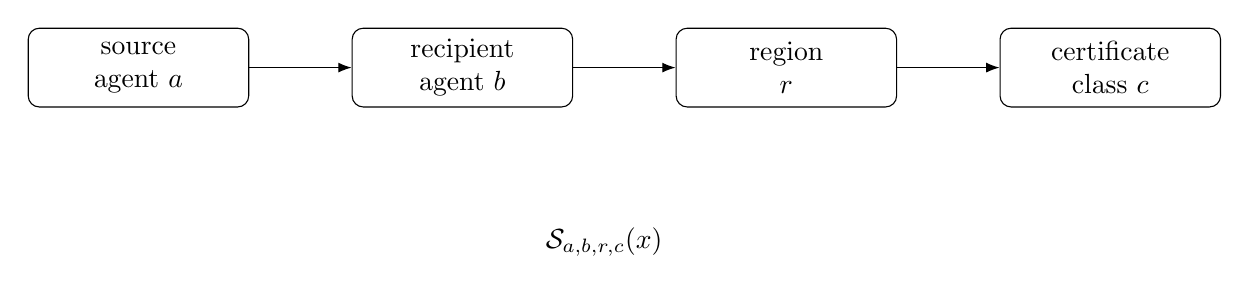
\begin{tikzpicture}[>=Latex,node distance=10mm and 13mm,box/.style={draw,rounded corners,align=center,minimum width=28mm,minimum height=10mm}]
\node[box] (a) {source\\agent $a$};
\node[box,right=of a] (b) {recipient\\agent $b$};
\node[box,right=of b] (r) {region\\$r$};
\node[box,right=of r] (c) {certificate\\class $c$};
\draw[->] (a)--(b); \draw[->] (b)--(r); \draw[->] (r)--(c);
\node[below=14mm of b,xshift=18mm] {$\mathcal S_{a,b,r,c}(x)$};
\end{tikzpicture}
\caption{One tensor entry asks who generated a discovery, who can use it, where it occurred, and which mutually exclusive terminal class it may advance.}
\end{figure}

\section{Constrained resource allocation}
Let $u=(u_1,\ldots,u_n)$ be computational allocations and let $B$ be total budget. Let $F_x(u)$ be a calibrated settlement objective inferred from the current state and tensor. The simplest problem is
\[
\max_{u\in\mathcal U}F_x(u),\qquad
\mathcal U=\{u:u_i\ge m_i,\ \sum_i u_i=B,\ Au\le b\}.
\]
The lower bounds $m_i$ can implement anti-starvation requirements for $P,R,I$, or other essential components.

\begin{proposition}[Existence]
If $\mathcal U$ is nonempty and compact and $F_x$ is continuous, then an optimal allocation exists.
\end{proposition}
\begin{proof}
This is the extreme-value theorem applied to $F_x$ on the compact feasible set $\mathcal U$.
\end{proof}

Ignoring inequalities momentarily, the Lagrangian for $\sum_i u_i=B$ is
\[
\mathcal L(u,\lambda)=F_x(u)-\lambda\left(\sum_i u_i-B\right).
\]
At an interior optimum,
\[
\frac{\partial F_x}{\partial u_i}=\lambda.
\]
Thus every actively funded channel has equal marginal expected settlement value at the optimum. The multiplier $\lambda$ is the shadow value of an additional unit of total computation. With inequality constraints the appropriate first-order framework is KKT \cite{boyd,kuhn}.

\begin{theorem}[Global KKT optimality under concavity]
Assume $\mathcal U$ is convex, $F_x$ is differentiable and concave, and a suitable constraint qualification such as Slater's condition holds. Then every feasible KKT point is a global maximizer of $F_x$. If $F_x$ is strictly concave, the maximizer is unique.
\end{theorem}

\section{An explicit diminishing-returns scheduler}
Consider
\[
F(u)=\sum_{i=1}^n w_i(1-e^{-a_i u_i}),\qquad w_i,a_i>0.
\]
Each summand is increasing and strictly concave. For an interior active channel,
\[
w_i a_i e^{-a_i u_i^*}=\lambda,
\]
so
\[
\boxed{u_i^*=\frac1{a_i}\log\left(\frac{w_i a_i}{\lambda}\right).}
\]
With lower bounds one clips this expression at $m_i$, and chooses $\lambda$ so that the budget constraint holds. This is a concrete water-filling-style scheduler.

\section{Quadratic tensor interactions and curvature}
A useful local model is
\[
F_x(u)=s(x)^Tu-\frac12u^TQ(x)u.
\]
If $Q(x)\succeq0$, then $\nabla^2F_x=-Q(x)\preceq0$ and the allocation problem is concave. If $Q(x)\succ0$, the optimum is unique. Strong positive cross-agent complementarities can make the Hessian indefinite, in which case KKT no longer guarantees a global optimum. The spectrum of the settlement Hessian is therefore a diagnostic for whether a current allocation problem lies in an easy concave regime or a harder nonconvex regime.

\section{Robustness to measurement error}
The true settlement objective is not observed directly. Suppose $\widehat F$ is an estimated objective satisfying
\[
\sup_{u\in\mathcal U}|\widehat F(u)-F(u)|\le\varepsilon.
\]
Let $u^*$ maximize $F$ and let $\widehat u$ maximize $\widehat F$.

\begin{theorem}[$2\varepsilon$ near-optimality]
\[
\boxed{F(u^*)-F(\widehat u)\le2\varepsilon.}
\]
\end{theorem}
\begin{proof}
Because $\widehat u$ maximizes $\widehat F$,
\[
\widehat F(\widehat u)\ge\widehat F(u^*).
\]
Uniform error then gives
\[
F(\widehat u)\ge\widehat F(\widehat u)-\varepsilon
\ge\widehat F(u^*)-\varepsilon
\ge F(u^*)-2\varepsilon.
\]
\end{proof}

If $F$ is $\mu$-strongly concave, then
\[
F(u^*)-F(\widehat u)\ge\frac\mu2\|\widehat u-u^*\|^2,
\]
so
\[
\boxed{\|\widehat u-u^*\|\le2\sqrt{\varepsilon/\mu}.}
\]
Thus a sufficiently well-calibrated imperfect tensor can still yield a quantitatively near-optimal resource allocation.

\section{Dynamic allocation}
Every verified discovery can change the bank, frontiers, and cross-agent value. Therefore $F_t$ and the optimal allocation $u_t^*$ move with time. A simple projected online update is
\[
u_{t+1}=\Pi_{\mathcal U}\bigl(u_t+\eta\nabla F_t(u_t)\bigr).
\]
Under bounded-domain and bounded-gradient assumptions, online gradient methods obtain sublinear static regret \cite{zinkevich}. If the optimum itself moves slowly, dynamic-regret analyses compare the controller to a moving benchmark.

For computation allocated one discrete quantum at a time, adaptive greedy policies become relevant when the expected utility satisfies adaptive monotonicity and adaptive submodularity \cite{golovin}.

\section{Connection to the proof-ocean compass}
The tensor is not itself the final navigator. One useful hierarchy is
\[
\text{local density and landmarks}
\longrightarrow \mathcal S(x)
\longrightarrow \widehat d_{\Sset}(x)
\longrightarrow \text{compass}
\longrightarrow \text{next tunnel}.
\]
On solved proof DAGs, exact distance to a terminal certificate provides an objective training label. Learning-guided ATP and progress-prediction work provide evidence that prior proofs and estimates of remaining proof progress can guide search \cite{enigmawatch,leanprogress}.

\begin{figure}[ht]
\centering
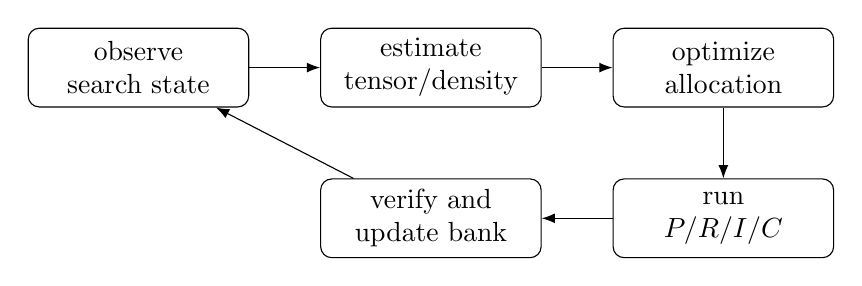
\begin{tikzpicture}[>=Latex,node distance=9mm and 9mm,box/.style={draw,rounded corners,align=center,minimum width=28mm,minimum height=10mm}]
\node[box] (obs) {observe\\search state};
\node[box,right=of obs] (ten) {estimate\\tensor/density};
\node[box,right=of ten] (opt) {optimize\\allocation};
\node[box,below=of opt] (run) {run\\$P/R/I/C$};
\node[box,left=of run] (ver) {verify and\\update bank};
\draw[->] (obs)--(ten); \draw[->] (ten)--(opt); \draw[->] (opt)--(run); \draw[->] (run)--(ver); \draw[->] (ver)--(obs);
\end{tikzpicture}
\caption{Closed-loop control. The optimizer chooses where computation goes; the verifier alone determines whether a mutually exclusive terminal class has actually been reached.}
\end{figure}

\section{What these results do and do not establish}
The results above conditionally solve parts of the AMLD resource-allocation meta-problem. They give sufficient conditions for existence, global KKT optimality, uniqueness, explicit allocation formulas, and robustness to objective-estimation error. They do not prove that an arbitrary target is reachable, decidable, or eventually settled. The central empirical task is calibration: determine whether tensor-derived measurements predict actual reductions in verified settlement cost on held-out proof oceans.

\section{Conclusion}
A consistent settlement optimizer must keep two layers separate. The terminal layer is discrete, one-hot, and verifier-gated. The navigation layer may be fractional, probabilistic, density-based, tensor-valued, and optimized continuously or discretely. This separation permits aggressive search guidance without weakening the meaning of mathematical settlement.

\begin{thebibliography}{9}
\bibitem{boyd} S. Boyd and L. Vandenberghe, \emph{Convex Optimization}. Cambridge University Press, 2004. \url{https://web.stanford.edu/~boyd/cvxbook/}
\bibitem{kuhn} H. W. Kuhn and A. W. Tucker, ``Nonlinear Programming,'' in \emph{Proceedings of the Second Berkeley Symposium on Mathematical Statistics and Probability}, 1951, pp. 481--492.
\bibitem{zinkevich} M. Zinkevich, ``Online Convex Programming and Generalized Infinitesimal Gradient Ascent,'' \emph{ICML}, 2003, pp. 928--936. \url{https://www.cs.cmu.edu/~maz/publications/ICML03.pdf}
\bibitem{golovin} D. Golovin and A. Krause, ``Adaptive Submodularity: Theory and Applications in Active Learning and Stochastic Optimization,'' \emph{JAIR} 42 (2011), 427--486. \url{https://arxiv.org/abs/1003.3967}
\bibitem{enigmawatch} Z. Goertzel, J. Jakub\r{u}v, and J. Urban, ``ENIGMAWatch: ProofWatch Meets ENIGMA,'' 2019. \url{https://arxiv.org/abs/1905.09565}
\bibitem{leanprogress} S. Huang, P. Song, R. J. George, and A. Anandkumar, ``LeanProgress: Guiding Search for Neural Theorem Proving via Proof Progress Prediction,'' 2025. \url{https://arxiv.org/abs/2502.17925}
\end{thebibliography}
\end{document}
